\documentclass[12pt, twoside]{article}
\usepackage[letterpaper, margin=1in, headsep=0.5in]{geometry}
\usepackage[english]{babel}
\usepackage[utf8]{inputenc}
\usepackage{amsmath}
\usepackage{amsfonts}
\usepackage{amssymb}
\usepackage{tikz}
\usepackage{yhmath}
\usetikzlibrary{quotes, angles}
\usepackage{graphicx}
\usepackage{enumitem}
\usepackage{multicol}

\newif\ifmeta
\metatrue %print standards and topics tags

\title{Regents Geometry}
\author{Chris Huson}
\date{May 2022}

\usepackage{fancyhdr}
\pagestyle{fancy}
\fancyhf{}
\renewcommand{\headrulewidth}{0pt} % disable the underline of the header
\raggedbottom

\fancyhead[LE]{\thepage}
\fancyhead[RO]{\thepage \\ Name: \hspace{4cm} \,\\}
\fancyhead[LO]{BECA / Dr. Huson / Geometry\\* Unit 11: Function transformations\\* 17 May 2022}

\begin{document}
\subsubsection*{11.14 Exit note: Perpendicular bisectors}
\begin{enumerate}
\item The line $l$ has the equation $y=-3x-2$.
  \begin{enumerate}
    \item What is the slope of line $l$?
    \vspace{0.5cm}
    \item Rewrite the equation of $l$ in the form $ax+by=c$.
    \vspace{1.3cm}
  \end{enumerate}

\item   
 \begin{enumerate}
  \item Find the slope $m$ of the line $3x-y=12$.
  \vspace{2cm}
  \item Write down the slope perpendicular to the line, $m_{\perp}$.
  \vspace{0.5cm}
\end{enumerate}

\item Write down the slope perpendicular to the given slope.
\begin{enumerate}
  \begin{multicols}{2}
    \item   $m= -\frac{3}{2} \hspace{1cm} m_{\perp} = $
    \item   $m= 2 \hspace{1cm} m_{\perp} = $ 
  \end{multicols}
\end{enumerate} \vspace{0.5cm}

\item The line segment $\overline{AB}$, $A(1,7)$ and $B(9,3)$, is shown below.
  \begin{multicols}{2}
    \begin{enumerate}
    \item Mark the midpoint $M$ of $\overline{AB}$. Label it as an ordered pair.
    \item Find the slope of $\overline{AB}$. \vspace{2cm}
    \item Write down the slope perpendicular to $\overline{AB}$. \vspace{1cm}
    \item Write down the equation of the perpendicular bisector of $\overline{AB}$. \vspace{2cm}
    \item Draw the perpendicular bisector on the graph.
  \end{enumerate} \vspace{1cm}  
  \begin{center} %4 quadrant regents grid
    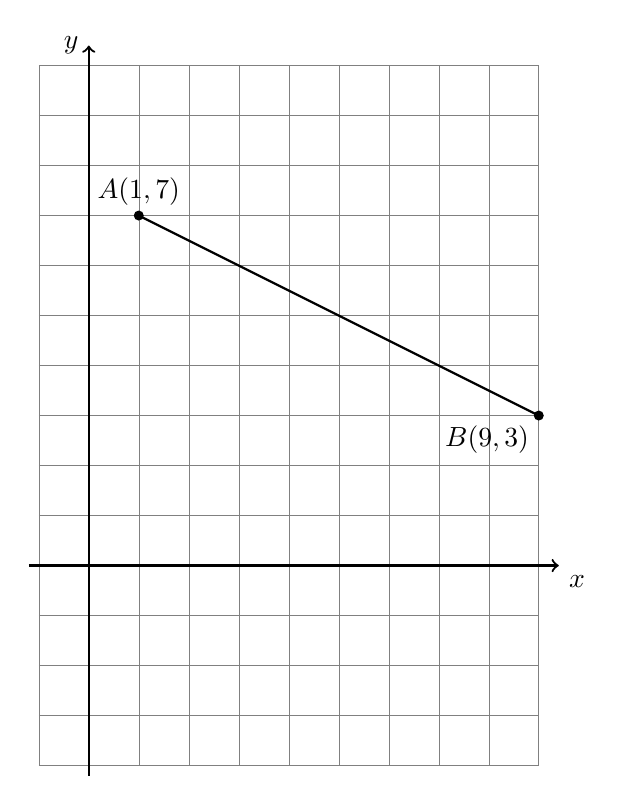
\begin{tikzpicture}[scale=.635]
      \draw [help lines] (-1,-4) grid (9,10);
      \draw [thick, ->] (-1.2,0) -- (9.4,0) node [below right] {$x$};
      \draw [thick, ->] (0,-4.2)--(0,10.4) node [left] {$y$};
      \draw [thick] (1,7)--(9,3);
      \fill (1,7) circle[radius=0.1cm]node[above]{$A(1,7)$};
      \fill (9,3) circle[radius=0.1cm]node[below left]{$B(9,3)$};
    \end{tikzpicture}
    \end{center} 
  \end{multicols}

\newpage
\item Write down the equation of the line through $(2,3)$ with a slope of $-2$.
\vspace{2cm}

\item The line $l$ has the equation $y-5=-3(x-2)$. Rewrite the  equation in slope-intercept form, $y=mx+b$. \vspace{3cm}

\item Quadrilateral $ABCD$ is shown on the graph below with $A(-1,-2)$, $B(5,2)$, $C(2,6)$, and $D(-4,2)$. Calculate the slopes of the four sides and show that $ABCD$ is a parallelogram but not a rectangle.
  \begin{flushright} %4 quadrant regents grid
  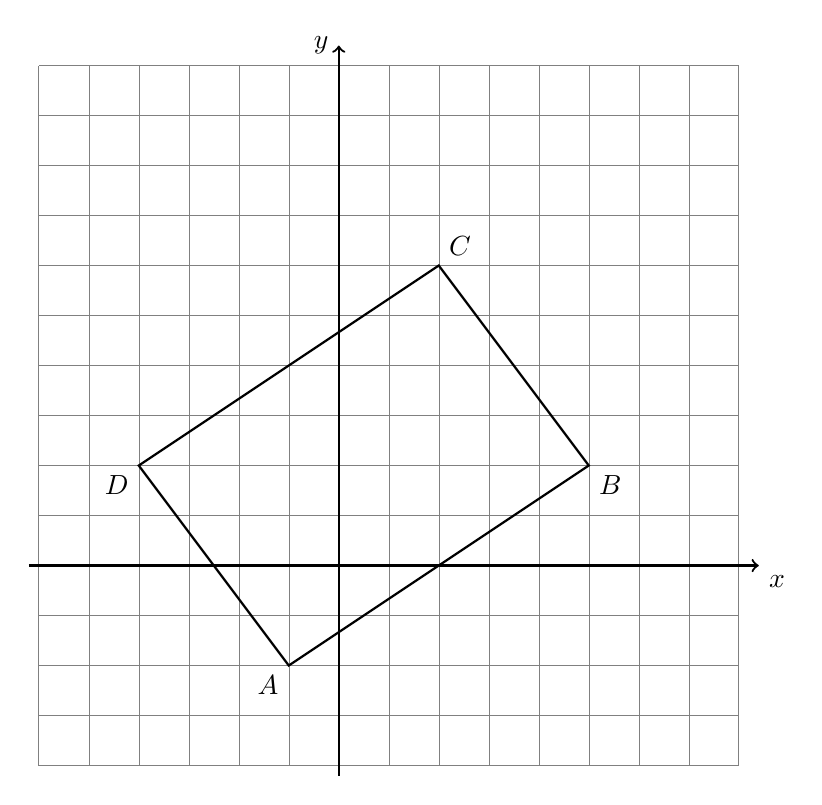
\begin{tikzpicture}[scale=.635]
    \draw [help lines] (-6,-4) grid (8,10);
    \draw [thick, ->] (-6.2,0) -- (8.4,0) node [below right] {$x$};
    \draw [thick, ->] (0,-4.2)--(0,10.4) node [left] {$y$};
    \draw [thick] (-1,-2)node[below left]{$A$}--
    (5,2)node[below right]{$B$}--
    (2,6)node[above right]{$C$}--
    (-4,2)node[below left]{$D$}--cycle;
  \end{tikzpicture}
  \end{flushright}

  
\end{enumerate}
\end{document}
